\documentclass{article}
\usepackage{graphicx}
\usepackage[dvipsnames,table]{xcolor}
\usepackage[utf8]{inputenc}
\usepackage{siunitx}
\usepackage[american,siunitx]{circuitikz}
\usepackage{amsmath}
\usepackage{svg}
\usepackage{booktabs}
\usepackage{float}
\usepackage{xparse, xfp}
\usepackage{multirow}
\usepackage{tikz}
\usepackage{karnaugh-map}
\usepackage{pdfpages}
\usepackage{hyperref}
\hypersetup{
    colorlinks=true,
    linkcolor=blue,
    filecolor=magenta,      
    urlcolor=cyan,
}
\usetikzlibrary{calc}
%\usepackage[landscape]{geometry}
\renewcommand{\thesubsection}{\thesection.\alph{subsection}}
\newcommand{\equal}{=}
\newcommand{\greyrule}{\arrayrulecolor{black!30}\midrule\arrayrulecolor{black}}
\makeatletter
\newcommand\currcoor{\the\tikz@lastxsaved,\the\tikz@lastysaved}
\makeatother
\newcolumntype{:}{@{\hskip\tabcolsep\color{black!30}\vrule\hskip\tabcolsep}}

\ExplSyntaxOn
\NewExpandableDocumentCommand \groupify { O{\,\allowbreak} m m }
  { \jakob_groupify:nnn {#1} {#2} {#3} }
\cs_new:Npn \jakob_groupify:nnn #1 #2 #3
  { \__jakob_groupify_loop:nnw { 1 } {#2} #3 \q_recursion_tail {#1} \q_recursion_stop }
\cs_new:Npn \__jakob_groupify_loop:nnw #1 #2 #3
  {
    \quark_if_recursion_tail_stop:n {#3}
    \exp_not:n {#3}
    \int_compare:nNnTF {#1} = {#2}
      { \__jakob_groupify_sep:n }
      { \exp_args:Nf \__jakob_groupify_loop:nnw { \int_eval:n { #1+1 } } }
          {#2}
  }
\cs_new:Npn \__jakob_groupify_sep:n #1 #2 \q_recursion_tail #3
  {
    \tl_if_empty:nF {#2} { \exp_not:n {#3} }
    \__jakob_groupify_loop:nnw { 1 } {#1}
    #2 \q_recursion_tail {#3}
  }
\ExplSyntaxOff

\title{ECE 2200L\\Introduction to Microelectronics Circuits Laboratory\\\,\\Experiment 2\\Diode I-V Characteristics\\\,\\Report}
\author{Choi Tim Antony Yung}
\begin{document}
\maketitle

\thispagestyle{empty}
\setcounter{page}{0}

\newpage

\section*{Objective}

To study the current-voltage relationship of semiconductor PN diodes, and to determine the reverse saturation current and the diode ideality factor from the I-V characteristic plot of the diodes.

\section*{Result}
\subsection*{1N4001 Silicon PN diode}
The following is the experimental data obtained from 1N4001 Silicon PN diode.
\begin{table}[H]
  \centering
    \begin{tabular}{rrrr}
    \toprule
    \multicolumn{1}{c}{$V_d$ (V)} & \multicolumn{1}{c}{$I_d$ (A)} & \multicolumn{1}{c}{$\frac{V_d}{V_T}$} & \multicolumn{1}{c}{$ln(I_d)$ (A)} \\
    \midrule
    -10   & $-2.000\times10^{-9}$ & \multicolumn{2}{c}{\multirow{5}[0]{*}{N/A}} \\
    -8    & $-2.000\times10^{-9}$ & \multicolumn{2}{c}{} \\
    -6    & $-2.000\times10^{-9}$ & \multicolumn{2}{c}{} \\
    -4    & $-2.000\times10^{-9}$ & \multicolumn{2}{c}{} \\
    -2    & $-1.000\times10^{-9}$ & \multicolumn{2}{c}{} \\
    0.3   & $ 9.000\times10^{-7}$ & 11.53846 & -13.9209 \\
    0.4   & $ 1.440\times10^{-5}$ & 15.38462 & -11.1483 \\
    0.5   & $ 1.910\times10^{-4}$ & 19.23077 & -8.56324 \\
    0.6   & $ 1.660\times10^{-3}$ & 23.07692 & -6.40094 \\
    0.7   & $ 1.407\times10^{-2}$ & 26.92308 & -4.26371 \\
    \bottomrule
  \end{tabular}
\end{table}

\begin{figure}[H]
  \centering
  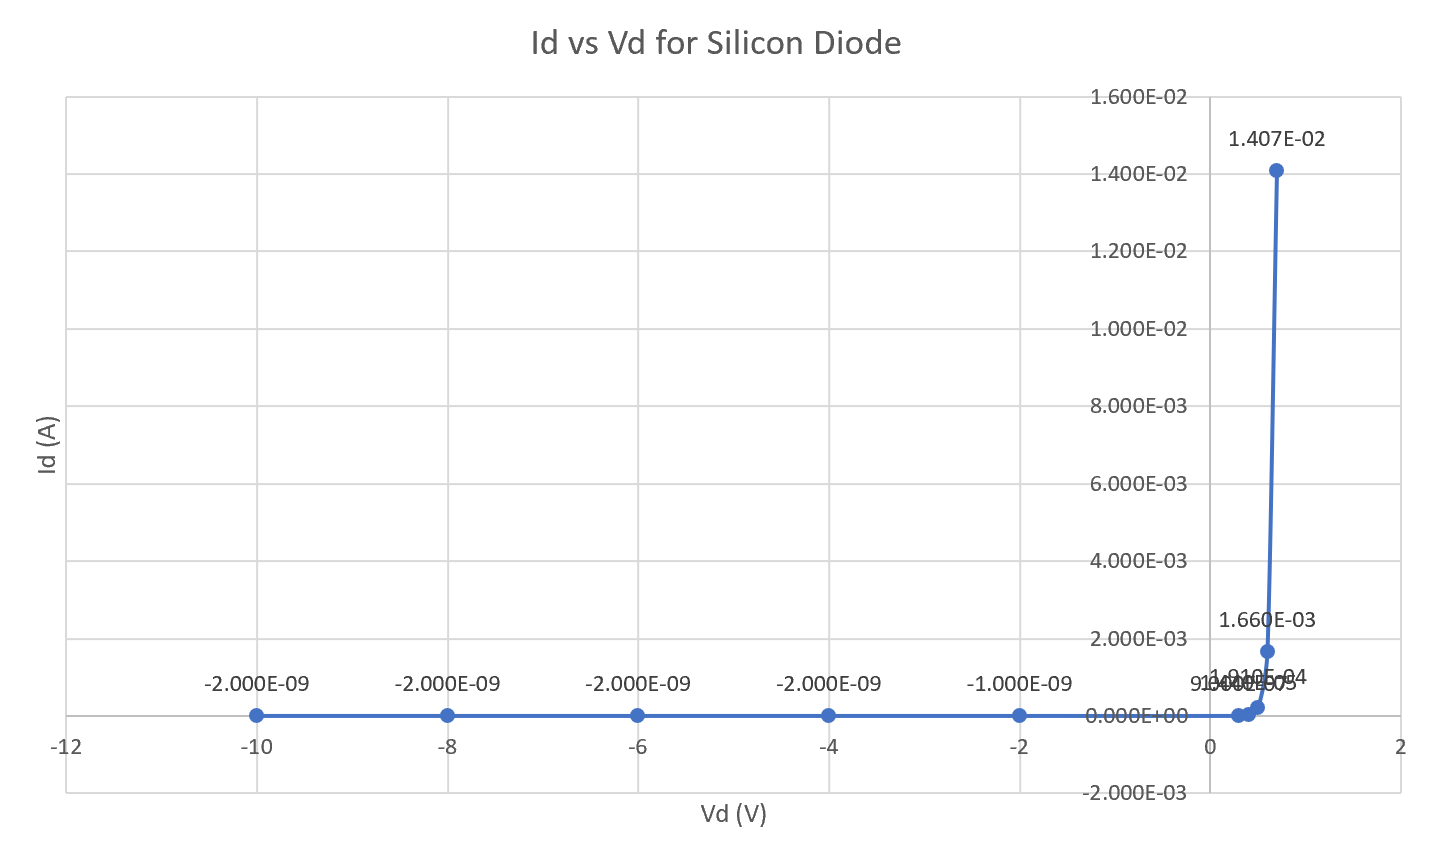
\includegraphics[width=\textwidth]{ECE2200L_Lab2_Si_IV.png}
  \caption{IV chart of 1N4001 Silicon PN diode}
\end{figure}
\begin{figure}[H]
  \centering
  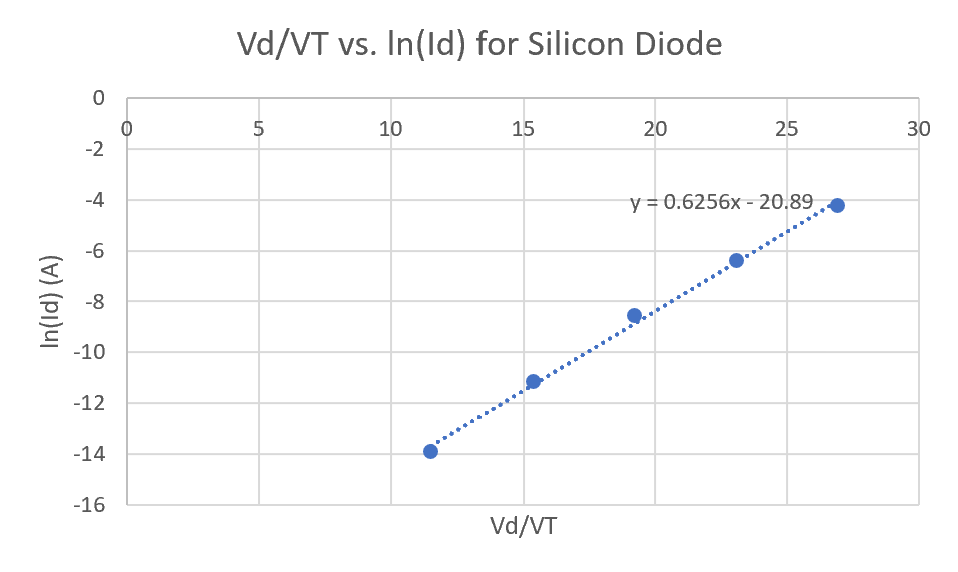
\includegraphics[width=\textwidth]{ECE2200L_Lab2_Si_log.png}
  \caption{$\frac{V_d}{V_T}$ vs $ln(I_d)$ chart of 1N4001 Silicon PN diode}
\end{figure}

From the above chart, the ideality of the diode $\eta$ can be derived by taking the reciprocal of the slope of the line of best fit and the saturation current $I_s$ can be derived by taking the inverse natural logarithm of the intercept of the line of best fit.

\begin{table}[H]
  \centering
    \begin{tabular}{rl}
    Slope & 0.6256 \\
    Intercept & \SI{-20.89}{\ampere} \\
    $\eta$     & 1.598465 \\
    $I_s$    & \SI{0.846}{\nano\ampere} \\
    \end{tabular}
\end{table}

\newpage

\subsection*{1N270 Germanium PN diode}
The following is the experimental data obtained from 1N270 Germanium PN diode.
\begin{table}[H]
  \centering
    \begin{tabular}{rrrr}
    \toprule
    \multicolumn{1}{c}{$V_d$ (V)} & \multicolumn{1}{c}{$I_d$ (A)} & \multicolumn{1}{c}{$\frac{V_d}{V_T}$} & \multicolumn{1}{c}{$ln(I_d)$ (A)} \\
    \midrule
    -10   & $-1.270\times10^{-6}$ & \multicolumn{2}{c}{\multirow{5}[0]{*}{N/A}} \\
    -8    & $-1.093\times10^{-6}$ & \multicolumn{2}{c}{} \\
    -6    & $-9.750\times10^{-7}$ & \multicolumn{2}{c}{} \\
    -4    & $-8.740\times10^{-7}$ & \multicolumn{2}{c}{} \\
    -2    & $-7.260\times10^{-7}$ & \multicolumn{2}{c}{} \\
    0.1   & $ 1.670\times10^{-5}$ & 3.846154 & -11.0001 \\
    0.2   & $ 2.220\times10^{-4}$ & 7.692308 & -8.41283 \\
    0.3   & $ 1.570\times10^{-3}$ & 11.53846 & -6.45668 \\
    0.4   & $ 7.550\times10^{-3}$ & 15.38462 & -4.88621 \\
    \bottomrule
  \end{tabular}
\end{table}

\begin{figure}[H]
  \centering
  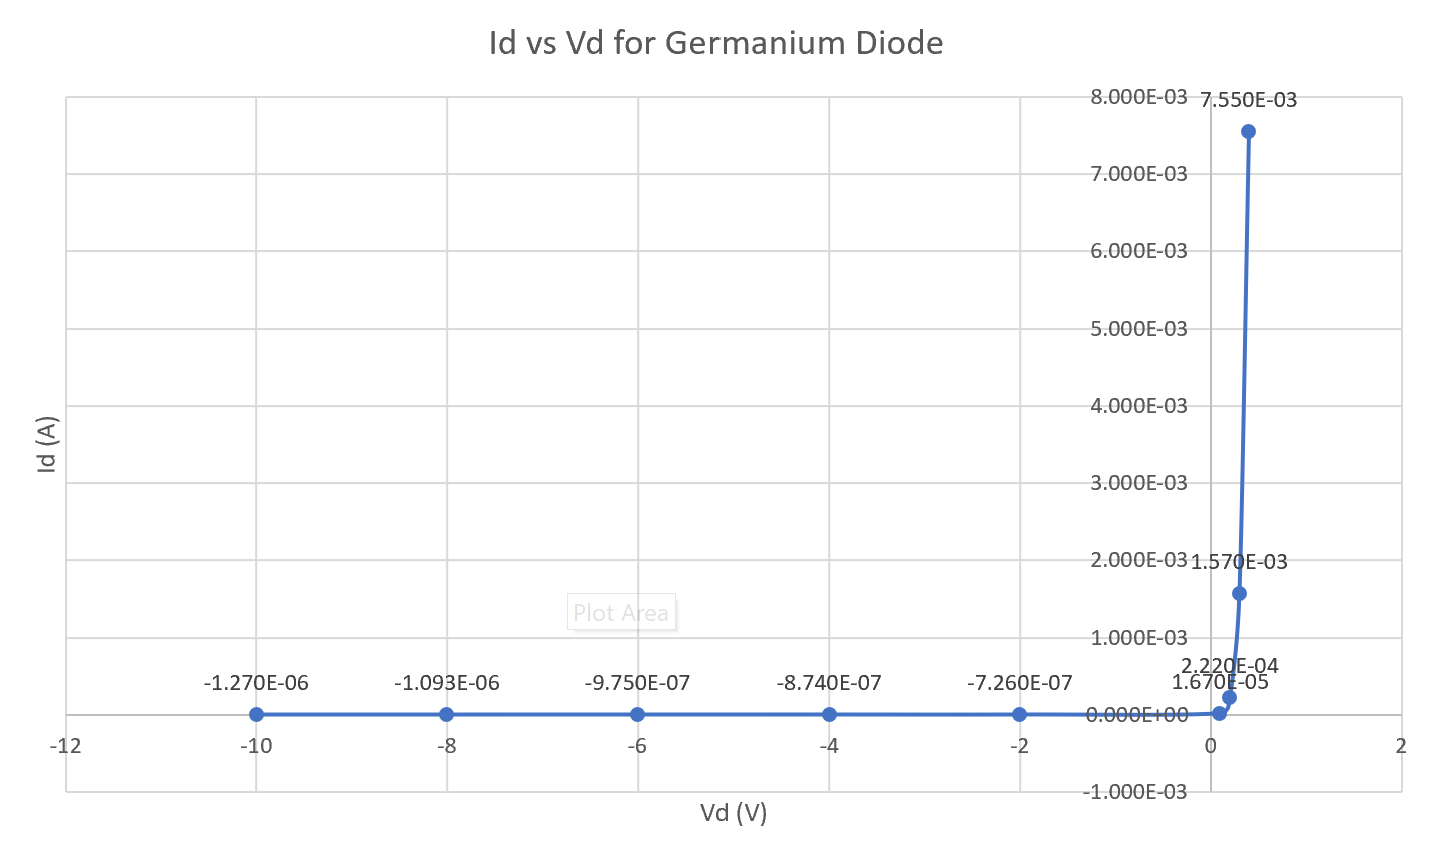
\includegraphics[width=\textwidth]{ECE2200L_Lab2_Ge_IV.png}
  \caption{IV chart of 1N270 Germanium PN diode}
\end{figure}
\begin{figure}[H]
  \centering
  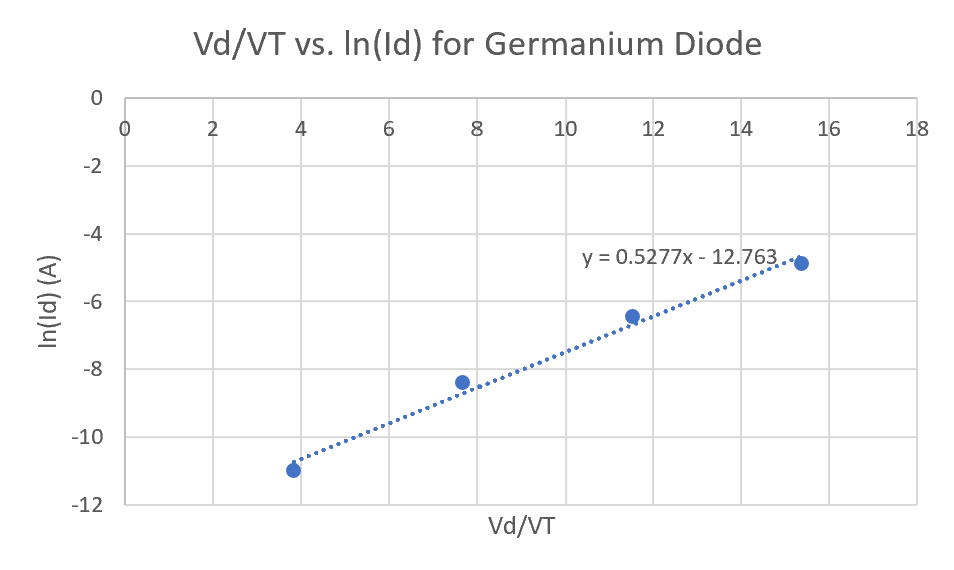
\includegraphics[width=\textwidth]{ECE2200L_Lab2_Ge_log.png}
  \caption{$\frac{V_d}{V_T}$ vs $ln(I_d)$ chart of 1N270 Germanium PN diode}
\end{figure}

From the above chart, the ideality of the diode $\eta$ can be derived by taking the reciprocal of the slope of the line of best fit and the saturation current $I_s$ can be derived by taking the inverse natural logarithm of the intercept of the line of best fit.

\begin{table}[H]
  \centering
    \begin{tabular}{rl}
    Slope & 0.5277 \\
    Intercept & \SI{-12.763}{\ampere} \\
    $\eta$     & 1.8950161 \\
    $I_s$    & \SI{2.86}{\micro\ampere} \\
    \end{tabular}
\end{table}

\section*{Conclusion}
The ideality factor of both Si and Ge diode derived from the $\frac{V_d}{V_T}$ vs $ln(I_d)$ plots are higher than expected. The increased temperature of diode when operating at relatively high voltage may have contributed to the higher value by increasing the thermal voltage, which is directly proportional to the calculation of ideality factor as it decreases the coefficient of the independant variable of the line derived from the $\frac{V_d}{V_T}$ vs $ln(I_d)$ plot, which is used to derive the ideality factor by taking the reciprocal of the slope, thus the decrease in slope resulted in an increase of ideality value derived.

\end{document}
